\documentclass[sigconf]{acmart}
\usepackage{algorithm}
\usepackage{algpseudocode}
\usepackage{comment}
\usepackage{subcaption}


% \setcopyright{acmlicensed}
% \copyrightyear{2024}
% \acmYear{2024}
% \acmDOI{XXXXXXX.XXXXXXX}

\acmConference{Geometry Data Analysis}{December 2024}{Paris, France}

\acmISBN{978-1-4503-XXXX-X/18/06}
\begin{document}
%%
%% The "title" command has an optional parameter,
%% allowing the author to define a "short title" to be used in page headers.
\title{Analysis over the Vector Heat Method}

%%
%% The "author" command and its associated commands are used to define
%% the authors and their affiliations.
%% Of note is the shared affiliation of the first two authors, and the
%% "authornote" and "authornotemark" commands
%% used to denote shared contribution to the research.
\author{Ícel Viñals Pierigé}
\affiliation{%
  \institution{\'Ecole nationale des Ponts et Chaussées}
  \city{Champs-sur-Marne}
  \country{France}}
\email{icel.vinals-pierige@enpc.fr}

\author{Cécile Liu}
\affiliation{%
  \institution{\'Ecole nationale des Ponts et Chaussées}
  \city{Champs-sur-Marne}
  \country{France}}
\email{cecile.liu@enpc.fr}

\author{Nicolas Sereyjol-Garros}
\affiliation{%
  \institution{\'Ecole nationale des Ponts et Chaussées}
  \city{Champs-sur-Marne}
  \country{France}}
\email{nicolas.sereyjol-garros@enpc.fr}


\begin{abstract}
  A clear and well-documented \LaTeX\ document is presented as an
  article formatted for publication by ACM in a conference proceedings
  or journal publication. Based on the ``acmart'' document class, this
  article presents and explains many of the common variations, as well
  as many of the formatting elements an author may use in the
  preparation of the documentation of their work.
\end{abstract}

%%
%% The code below is generated by the tool at http://dl.acm.org/ccs.cfm.
%% Please copy and paste the code instead of the example below.
%%
\begin{CCSXML}
<ccs2012>
   <concept>
       <concept_id>10010147.10010371.10010396.10010402</concept_id>
       <concept_desc>Computing methodologies~Shape analysis</concept_desc>
       <concept_significance>500</concept_significance>
       </concept>
   <concept>
       <concept_id>10002950.10003714.10003715.10003750</concept_id>
       <concept_desc>Mathematics of computing~Discretization</concept_desc>
       <concept_significance>500</concept_significance>
       </concept>
   <concept>
       <concept_id>10002950.10003714.10003727.10003729</concept_id>
       <concept_desc>Mathematics of computing~Partial differential equations</concept_desc>
       <concept_significance>500</concept_significance>
       </concept>
 </ccs2012>
\end{CCSXML}

\ccsdesc[500]{Computing methodologies~Shape analysis}
\ccsdesc[500]{Mathematics of computing~Discretization}
\ccsdesc[500]{Mathematics of computing~Partial differential equations}

%%
%% Keywords. The author(s) should pick words that accurately describe
%% the work being presented. Separate the keywords with commas.
\keywords{discrete differential geometry, parallel
transport, velocity extrapolation, logarithmic map, exponential map, Karcher
mean, geometric median}

\received{20 February 2007}
\received[revised]{12 March 2009}
\received[accepted]{5 June 2009}

%%
%% This command processes the author and affiliation and title
%% information and builds the first part of the formatted document.
\maketitle

\section{Introduction}

\section{Context}
(nicolas)

\section{Methodologies}
\subsection{Vector heat method}
The vector heat method is presented in algorithm \ref{algo1}: the vector heat equation is used to diffuse the input vector field and then the scalar heat vector is used to adjust the magnitude of the resulting vectors. Indeed, the vector heat equation gives vectors pointing to the right directions for small values of time $t$ but the magnitudes are wrong. 

\begin{algorithm}
\caption{Vector Heat Method} \label{algo1}
\begin{algorithmic}
\Require A vector field $X$ supported on a subset $\Omega \subset M$ of the domain $M$.
\Ensure A vector field $\overline{X}$ on all of $M$.
%\Input{A vector field $X$ supported on a subset $\Omega \subset M$ of the domain $M$.}
%\Output{A vector field $\overline{X}$ on all of $M$.}

\noindent \textbf{I.} Integrate the vector heat flow $\frac{d}{dt} Y_t = \Delta Y_t$ for time $t$, with $Y_0 = X$. \\

\textbf{II.} Integrate the scalar heat flow $\frac{d}{dt} u_t = \Delta u_t$ for time $t$, with $u_0 = |X|$. \\

\textbf{III.} Integrate the scalar heat flow $\frac{d}{dt} \phi_t = \Delta \phi_t$ for time $t$, with $\phi_0 = \mathbf{1}_{\Omega}$. \\

\textbf{IV.} Evaluate the vector field $\overline{X}_t = \frac{u_t Y_t}{\phi_t |Y_t|}$.
\end{algorithmic}
\end{algorithm}

\subsubsection{Step 1: get the right directions}
As mentioned earlier, the idea of the vector heat method is to use the vector heat equation 
\begin{equation} \label{eq:vector-heat}
  \frac{d}{dt} X_t = \Delta^\nabla X_t
  \end{equation}
to diffuse the initial vector field. The symbol $\Delta^\nabla$ denotes the connection Laplacian associated to the Levi-Civita connection $\nabla$. 
We now consider a fundamental solution to the heat equation: the \textbf{heat kernel} denoted by $k_t^\nabla$. $k_t^\nabla(x,y)$ describes how 
a vector at a single point $x$ will diffuse to all other points $y$ over time $t$. For $y$ not on the cut locus of $x$, the following asymptotic
expansion holds:
\begin{equation} \label{eq:asymptotic_expansion}
  k_t^\nabla(x, y) \sim \frac{e^{-\frac{d(x, y)^2}{4t}}}{(4 \pi t)^{n/2} j(x, y)^\frac{1}{2}} 
\left( \sum_{i=0}^{\infty} t^i \Psi_i(x, y) \right)
  \end{equation}
\subsubsection{Step 2: get the right magnitudes}
\begin{comment}
\begin{algorithm}
\caption{An algorithm with caption}\label{alg:cap}
\begin{algorithmic}
\Require $n \geq 0$
\Ensure $y = x^n$
\State $y \gets 1$
\State $X \gets x$
\State $N \gets n$
\While{$N \neq 0$}
\If{$N$ is even}
    \State $X \gets X \times X$
    \State $N \gets \frac{N}{2}$  \Comment{This is a comment}
\ElsIf{$N$ is odd}
    \State $y \gets y \times X$
    \State $N \gets N - 1$
\EndIf
\EndWhile
\end{algorithmic}
\end{algorithm}
\end{comment}

\section{Experiences}
\subsection{Introduction}

\subsection{Our set-up}
(icel)
To realise these experiences, we first tested the C++ demo presented in the paper's website.
In this demo, the solvers for the scalar and vector heat methods were implemented in a library named Geometry Central.
To simplify the experimentation and work in a more familiar set-up, we used instead a Python library equivalent named Potpourri3d \cite{library_potpourri3d}, 
which was developped by one of the authors of the paper.
In addition to this, we used Trimesh for the manipulation of meshes and PyVision to visualize the results.

For the 3d bodies used throught the experiment, we started with those in the github repository~\cite{github_objects_repo},
as they presented clean 3d manifolds.

\subsection{Scalar heat robustness}
(icel)
The first experience we did was to analyze the robustness of the Scalar Heat Method~\cite{Crane:2017:HMD}. In
the original paper, the authors tested different noise types: missing and sliver triangles,
noisy coordinates and smoothed surfaces. So we recreated similar perturbations and numerically
measured the results.

For this numerical representation, we decided to compare two things. First, the original body
with an exact slower method from the gdist library~\cite{exact_method_algorithm}\cite{exact_method_library}
against the noisy body with the scalar heat method.
Then, the noisy body with the exact method against the noisy body with the scalar heat method again.
The first values explain the imperfections comming from the inexact method and the noise, while
the second only tests the behaviour of our method in a noisy environment.

Given $M = (V, F)$ our original mesh, $N = |V|$ the number of vertices in the mesh, $\hat{M} = (\hat{V}, \hat{F})$ the formulas used for this representation were:

\begin{equation} \label{eq:nvn_precision}
  \text{precision}_{\text{noisy v noisy}} = \frac{\sum_{i=1}^N \mathbf{1}_{\{|\text{dist}_1(\hat{V}_i) - \text{dist}_2(\hat{V}_i)| < 2\%\}}}{\text{N}} 
\end{equation}

\begin{equation} \label{eq:ovn_precision}
  \text{precision}_{\text{original v noisy}} = \frac{\sum_{i=1}^N \mathbf{1}_{\{|\text{dist}_1(V_i) - \text{dist}_2(\hat{V}_i)| < 2\%\}}}{\text{N}} 
\end{equation}

Where $\text{dist}_1$ and $\text{dist}_2$ are both the normalized distances (from 0 to 1 for the intrinsic farthest point) obtained from the exact method and the shm respectively.

We tested the robustness with two different type of noises (Fig~\ref{fig:all_bunnies}), inspired from what was presented in the paper. 
The first one is a gaussian perturbation of the position of all vertices. The variation of this noise was the noise level times the average edge length.
The second noise was a triangle swapp and triangle removal of a percentage of all triangles.
The triangle swap is simply to find a pair of faces $abc$, $bcd$ and convert them to $abd$ and $acd$.
This last perturbation quickly degenerated the meshes to the point where the exact algorithm could not
process the geodesic distances, so it was keept to a smaller noise level. 

To have a more general analysis, we used three different meshes and a set of ten random
source points. The meshes from the repo~\cite{github_objects_repo} were, in order of complexity, cow (5.8k triangles), the Stanford Bunny (69.5k triangles) and Horse (97k triangles).

In fig~\ref{fig:original_vs_noisy} we have the precision of the shm method on noisy mesh compared with the exact method in the original mesh for
different levels of gaussian noise, while in fig~\ref{fig:noisy_vs_noisy} we compare both methods only in the noisy objects.

We can see for the the large meshes the precision starts being virtually perfect, but it
decays gradually with the noise increases, this appears only on the first graph, as if we compare it to the noisy vs noisy, the precision
only decays slightly for the noisiest tests. We can understand that most of these errors come from comparing the original and the noisy objects
and do not depend on the method used.

For smaller meshes, where the edge-length body-length ratio is more significant, we have that the precision is generally smaller,
and even comparing both methods on the same noisy object gives a more significant number of inaccuracies, ranging from 10\% for the
original object to 30\% for the largest noise levels.

Analyzing the errors for the swapped and missing faces noise we plot our results
in fig~\ref{fig:noisy_vs_noisy_swapped_and_removed}. We see that SHM is virtually perfect
for larger meshes, but again the noise on the smaller model is more significant because
of its simplicity, what leads to some imprecisions. 

\begin{figure}
  \centering
  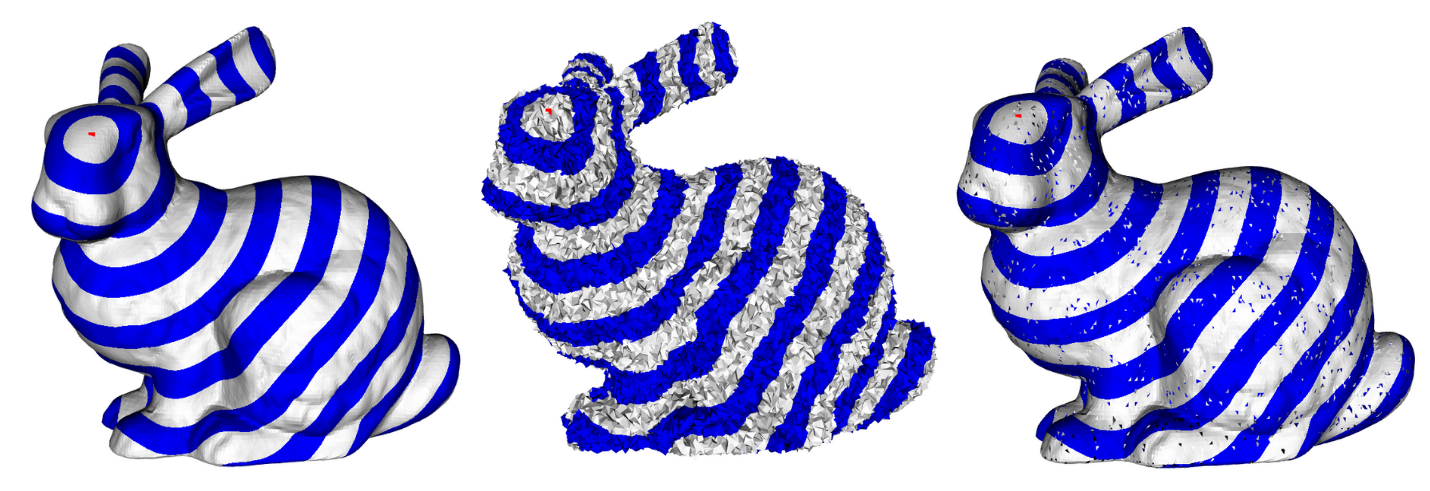
\includegraphics[width=8cm]{all_bunnies.png}
  \caption{From left to right we have the original stanford-bunny, the gaussian noised (50\% of average edge length) and a triangle swapped and removed noise (5\% of all triangles affected)}
  \label{fig:all_bunnies}
\end{figure}

\begin{figure}[htbp]
  \centering
  \hfill
  \begin{subfigure}[b]{0.23\textwidth}
    \centering
    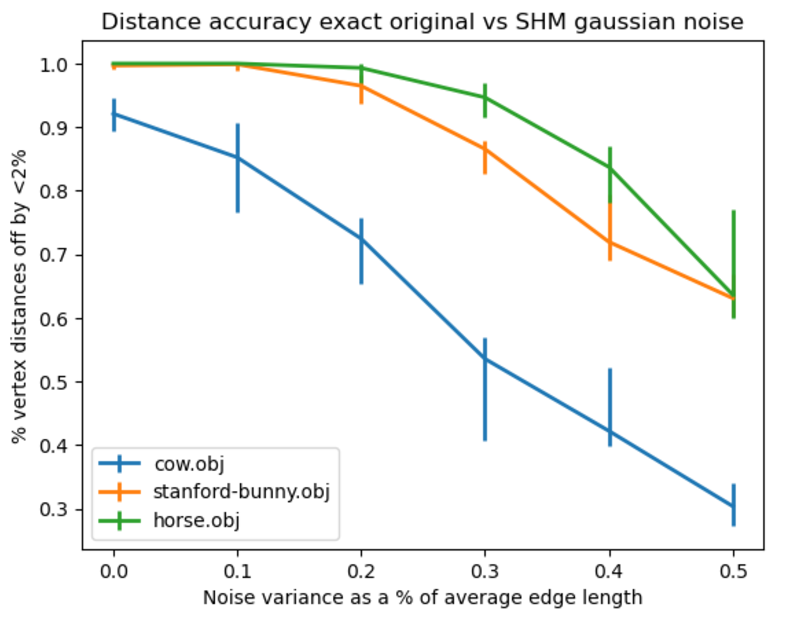
\includegraphics[width=\textwidth]{original_vs_noisy.png}
    \caption{Original vs noisy meshes}
    \label{fig:original_vs_noisy}
  \end{subfigure}
  \begin{subfigure}[b]{0.23\textwidth}
    \centering
    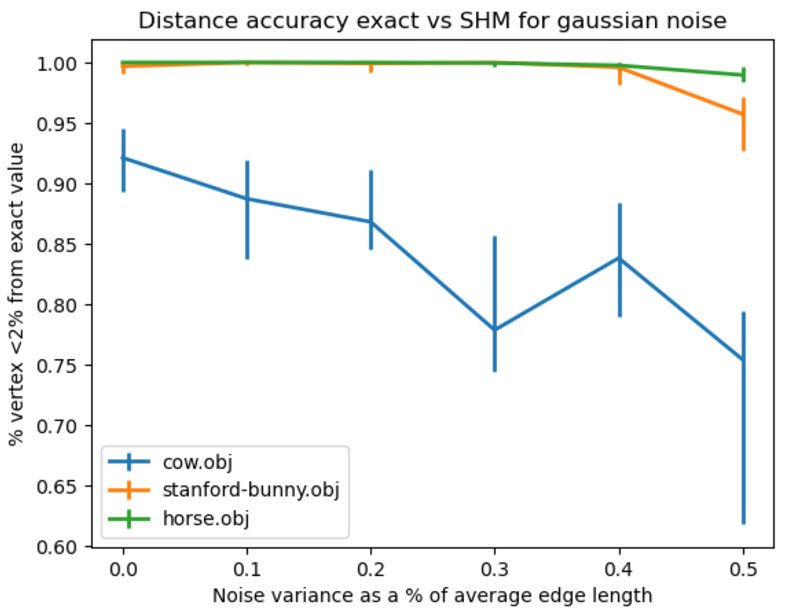
\includegraphics[width=\textwidth]{noisy_vs_noisy.png}
    \caption{Noisy vs noisy meshes}
    \label{fig:noisy_vs_noisy}
  \end{subfigure}
  \caption{Precision comparison with Gaussian noise}
  \label{fig:original_vs_noisy_gaussian}
\end{figure}

\begin{figure}
  \centering
  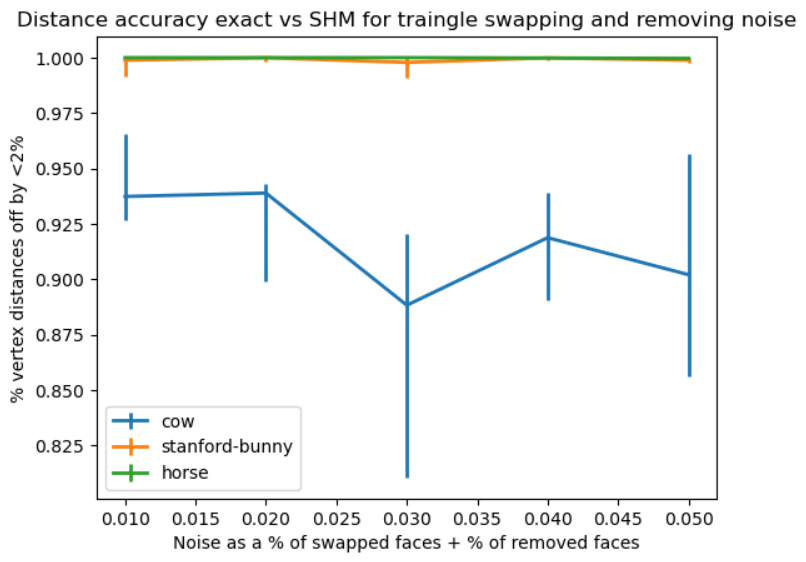
\includegraphics[width=8cm]{original_vs_original_swapped_and_removed_triangles.png}
  \caption{Noisy vs noisy meshes for swapped and removed faces noise type}
  \label{fig:noisy_vs_noisy_swapped_and_removed}
\end{figure}

Lastly, one type of noise for triangle meshes that was not introduced in the paper comes from
wrongly connected faces (Fig~\ref{fig:hands}). The algorithm presented is not inmune to these errors,
as it gives a correct representation of the distance for the perturbed mesh. So the method
presented is relatively robust to noise, but it still necesitates a curated mesh as its input. 

One possible solution to this is to take a point cloud instead, if the manifold represented is
dense enough, it will give a correct representation of the distances (Fig~\ref{fig:hand_distances}).

\begin{figure}
  \centering
  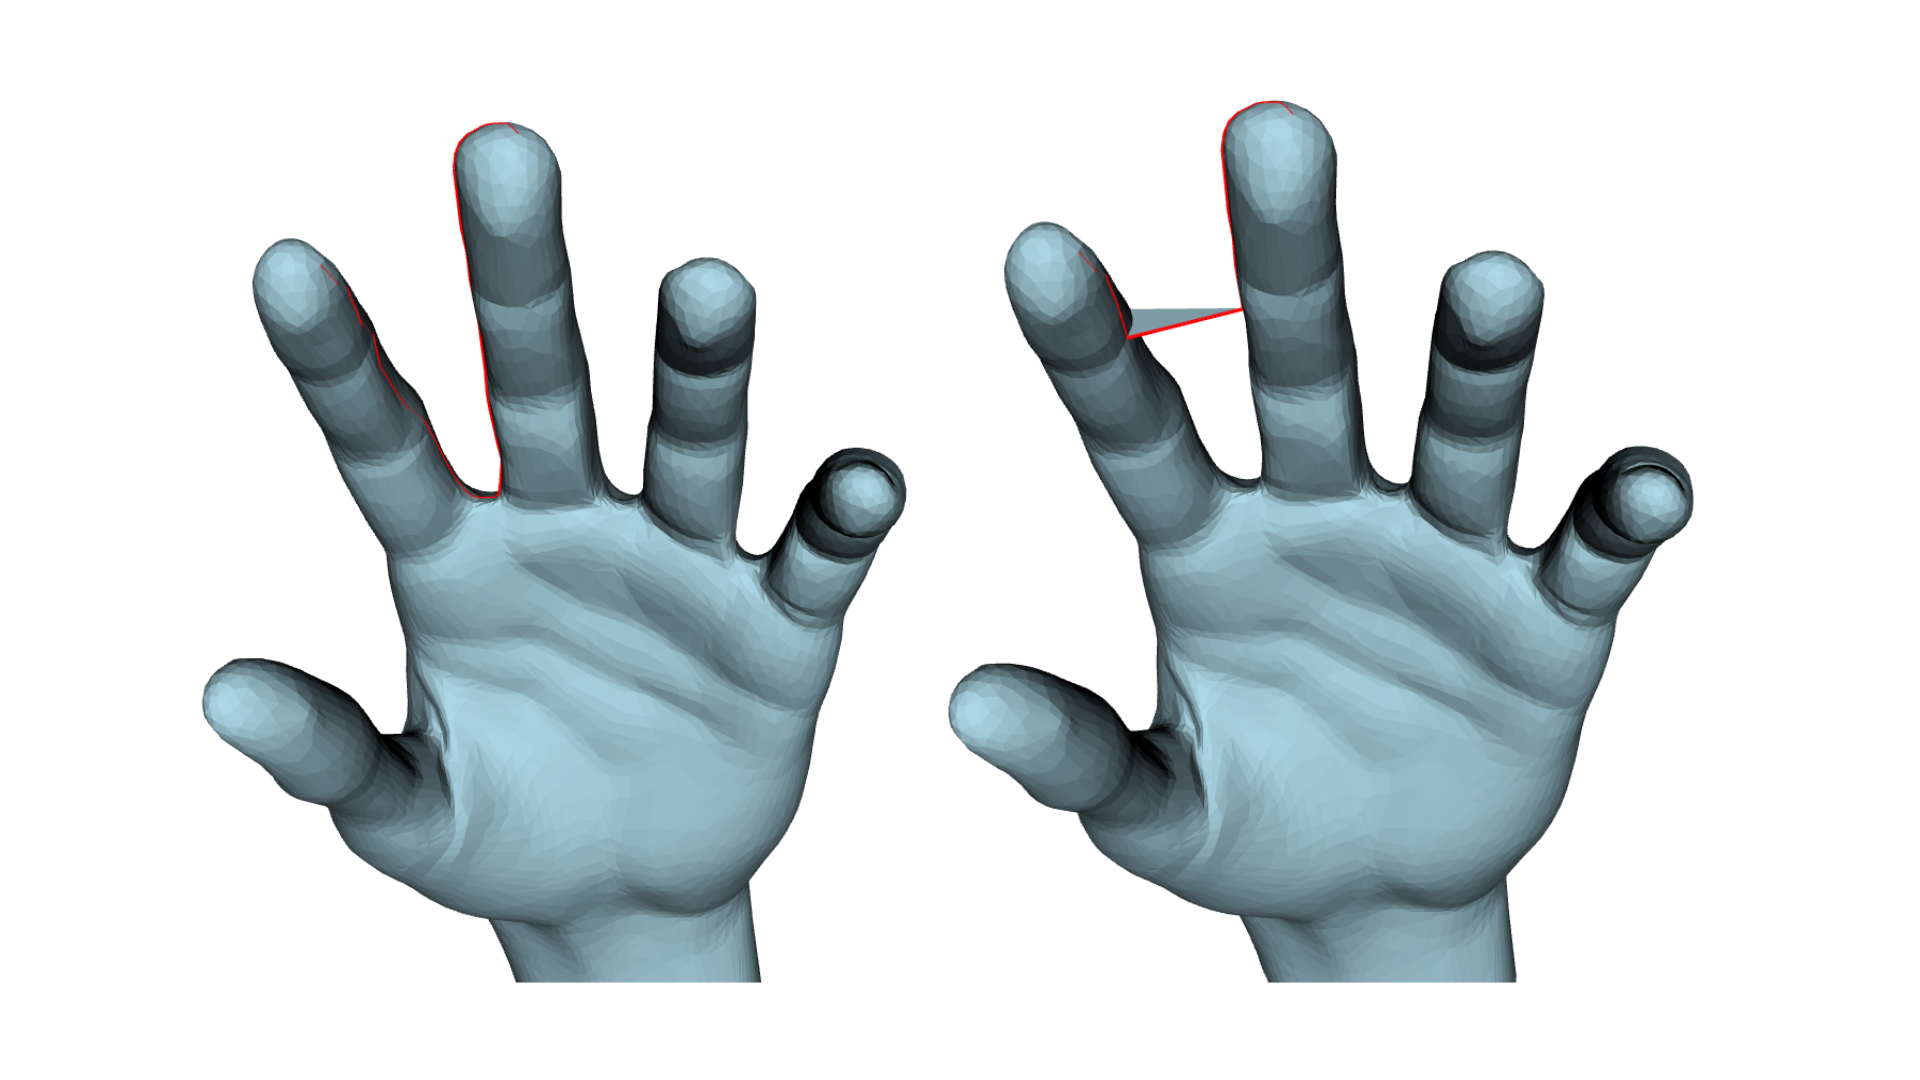
\includegraphics[width=8cm]{hands.png}
  \caption{Shortest path from finger to finger with and without an crossed extra face}
  \label{fig:hands}
\end{figure}

\begin{figure}
  \centering
  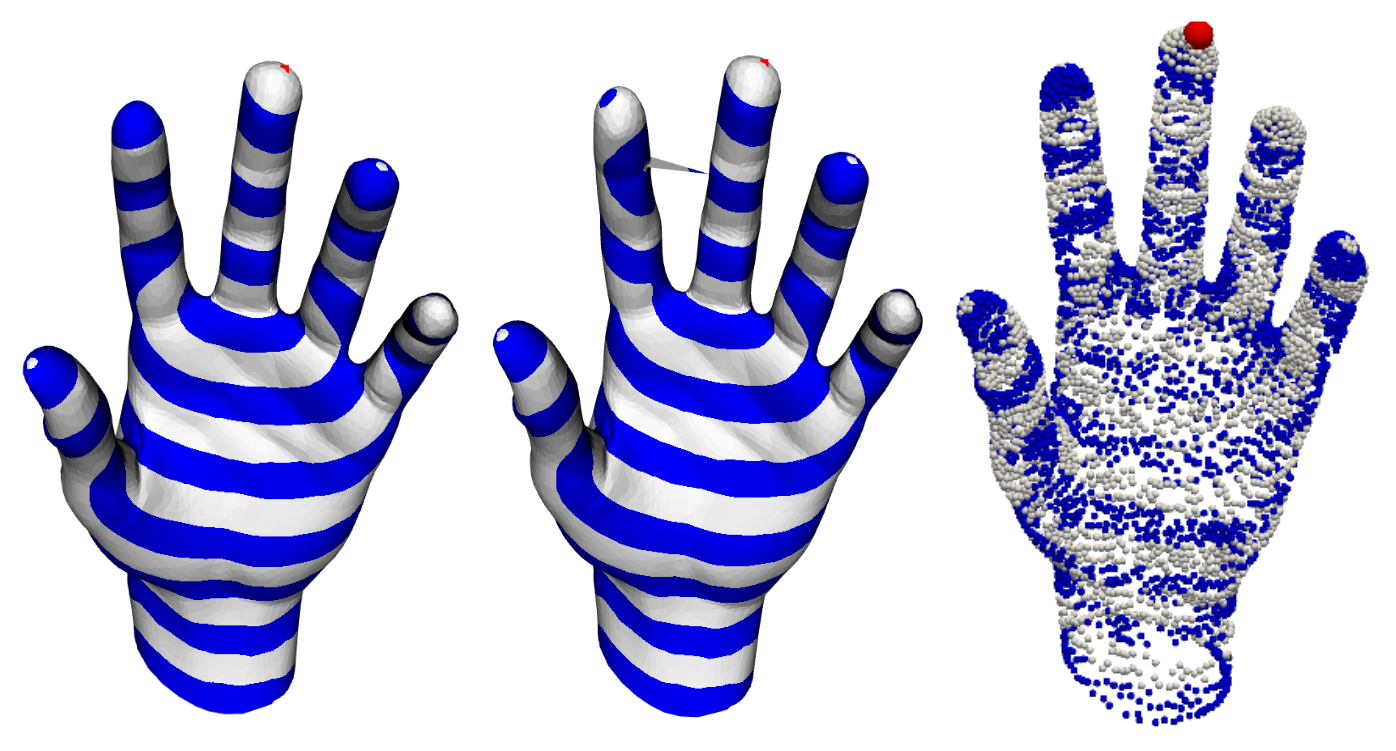
\includegraphics[width=8cm]{hands_distances.png}
  \caption{Distances from fingertip in original hand mesh, perturbed mesh and point cloud}
  \label{fig:hand_distances}
\end{figure}

\subsection{T's verifications with perfect results}
(nicolas)
https://hhoppe.com/geodesics.pdf

\subsection{Behavior at cut locus}
(cécile)
\subsection{Log-map recreation for postures}

\subsection{Preprocessing vs processing times}
(icel)

The implementation of the SHM algorithm is composed of two parts,
a preprocessing to get the laplacians and the computation of the 
distances from a source vertex/set of vectors.

In this point we wanted to compare the speed of this method with
the exact method using meshes of different sizes. For the experiment,
we ran three experiments, first measure the time for the exact method,
then measure the time for the SHM executing the preprocessing and processing
every loop, and finally executing the SHM preprocessing once and then computing
the distances in the loop.

We plotted the results obtained in fig~\ref{fig:time_graphs}. We can see that
for the larger plots the exact algorithm is slower than the SHM. However, almost all
time is dedicated to the preprocessing of the mesh, so the improvements are not so

If we could only use the FMM in python...

\begin{figure}
  \centering
  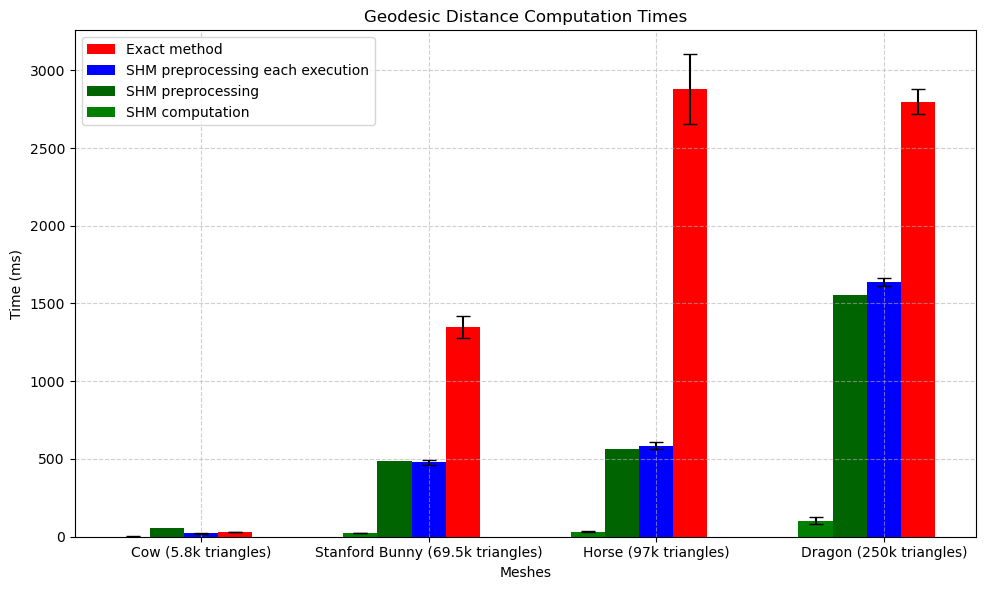
\includegraphics[width=8cm]{time_graphs.png}
  \caption{Times measured}
  \label{fig:time_graphs}
\end{figure}




\section{BRAIN STORM:}
\begin{itemize}
  \item Test robustness with a custom mesh + noise (similar to what they did) and mesh+crossed triangles (shortcuts should break the results?)
  \item Test different step sizes (t's) verify that 1 seems to be the best
  \item Compare results numerically with 'perfect' algorithm from https://hhoppe.com/geodesics.pdf
  \item Find how to test with different data types (point clouds, triang meshes, poly meshes) and compare results (if possible in software without too much rewriting?)
  \item Try results on bad vs good triangulated meshes (to check if Delaunay works fine)
  \item Think about new possible applications? Videogames/3d animation?? 
  \item Check 2020 method to compute geodesics only by flipping triangles. One advantage seems to be that it works to find not only global shortest paths, but also local ones (if two points are next to each other, it can find the shortest path in the opposite direction by turning around)  https://dl.acm.org/doi/10.1145/3414685.3417839
  \item Test speed against fast marching method for scalar heat method
  \item Check behaviour at Cut locus and comment it
  \item Look for applications the Karcher mean
\end{itemize}

\bibliographystyle{ACM-Reference-Format}
\bibliography{sample-base}


\end{document}

\endinput
%%
%% End of file `sample-sigconf-authordraft.tex'.
